% Credits are indicated where needed. The general idea is based on a template by Vel (vel@LaTeXTemplates.com) and Frits Wenneker.

\documentclass[11pt, a4paper]{article} % General settings in the beginning (defines the document class of your paper)
% 11pt = is the font size
% A4 is the paper size
% “article” is your document class

%----------------------------------------------------------------------------------------
%	Packages
%----------------------------------------------------------------------------------------

% Necessary
\usepackage[german,english]{babel} % English and German language 
\usepackage{hyperref} % URL
\usepackage{listings} % Insert code
\usepackage{lipsum}
\usepackage{mwe}
\usepackage{booktabs} % Horizontal rules in tables 
% For generating tables, use “LaTeX” online generator (https://www.tablesgenerator.com)
\usepackage{comment} % Necessary to comment several paragraphs at once
\usepackage[utf8]{inputenc} % Required for international characters
\usepackage[T1]{fontenc} % Required for output font encoding for international characters

% Might be helpful
\usepackage{amsmath,amsfonts,amsthm} % Math packages which might be useful for equations
\usepackage{tikz} % For tikz figures (to draw arrow diagrams, see a guide how to use them)
\usepackage{tikz-cd}
\usetikzlibrary{positioning,arrows} % Adding libraries for arrows
\usetikzlibrary{decorations.pathreplacing} % Adding libraries for decorations and paths
\usepackage{tikzsymbols} % For amazing symbols ;) https://mirror.hmc.edu/ctan/graphics/pgf/contrib/tikzsymbols/tikzsymbols.pdf 
\usepackage{blindtext} % To add some blind text in your paper


%---------------------------------------------------------------------------------
% Additional settings
%---------------------------------------------------------------------------------

%---------------------------------------------------------------------------------
% Define your margins
\usepackage{geometry} % Necessary package for defining margins

\geometry{
	top=2cm, % Defines top margin
	bottom=2cm, % Defines bottom margin
	left=2.2cm, % Defines left margin
	right=2.2cm, % Defines right margin
	includehead, % Includes space for a header
	%includefoot, % Includes space for a footer
	%showframe, % Uncomment if you want to show how it looks on the page 
}

\setlength{\parindent}{15pt} % Adjust to set you indent globally 

%---------------------------------------------------------------------------------
% Define your spacing
\usepackage{setspace} % Required for spacing
% Two options:
\linespread{1.5}
%\onehalfspacing % one-half-spacing linespread

%----------------------------------------------------------------------------------------
% Define your fonts
\usepackage[T1]{fontenc} % Output font encoding for international characters
\usepackage[utf8]{inputenc} % Required for inputting international characters

\usepackage{XCharter} % Use the XCharter font


%---------------------------------------------------------------------------------
% Define your headers and footers

\usepackage{fancyhdr} % Package is needed to define header and footer
\pagestyle{fancy} % Allows you to customize the headers and footers

%\renewcommand{\sectionmark}[1]{\markboth{#1}{}} % Removes the section number from the header when \leftmark is used

% Headers
\lhead{} % Define left header
\chead{\textit{}} % Define center header - e.g. add your paper title
\rhead{} % Define right header

% Footers
\lfoot{} % Define left footer
\cfoot{\footnotesize \thepage} % Define center footer
\rfoot{ } % Define right footer

%---------------------------------------------------------------------------------
%	Add information on bibliography
\usepackage{natbib} % Use natbib for citing
\usepackage{har2nat} % Allows to use harvard package with natbib https://mirror.reismil.ch/CTAN/macros/latex/contrib/har2nat/har2nat.pdf

% For citing with natbib, you may want to use this reference sheet: 
% http://merkel.texture.rocks/Latex/natbib.php

%---------------------------------------------------------------------------------
% Add field for signature (Reference: https://tex.stackexchange.com/questions/35942/how-to-create-a-signature-date-page)
\newcommand{\signature}[2][5cm]{%
  \begin{tabular}{@{}p{#1}@{}}
    #2 \\[2\normalbaselineskip] \hrule \\[0pt]
    {\small \textit{Signature}} \\[2\normalbaselineskip] \hrule \\[0pt]
    {\small \textit{Place, Date}}
  \end{tabular}
}
%---------------------------------------------------------------------------------
%	General information
%---------------------------------------------------------------------------------
\title{Deep Learning HW2 Report} % Adds your title
%\author
%{
%    \name{Alfons Hwu} % Add your first and last name
%    %\thanks{} % Adds a footnote to your title
%    \\
%    \institution{0416324, Dept of Computer Science NCTU} % Adds your institution
%}



%---------------------------------------------------------------------------------
%	Define what’s in your document
%---------------------------------------------------------------------------------
\begin{document}


% If you want a cover page, uncomment "%---------------------------------------------------------------------------------
% Cover page
%---------------------------------------------------------------------------------

% Here are more templates for other cover pages: https://www.latextemplates.com/cat/title-pages

% This example is based on this cover page example: https://www.latextemplates.com/template/academic-title-page

\begin{titlepage} % Starts new environment where the page number is not displayed and the count starts at 1 for the next page

%------------------------------------------------
%	Institutional information
%------------------------------------------------
	
\begin{minipage}{0.4\textwidth} % Begins new environment (like a text box)
    \begin{flushleft} % Sets environment on the left side of the paper
    \large
    National Chiao Tung University\\ % Add your institution
    Spring 2019 \\ % Add term
    Deep Learning \\ % Add course title
    Instructor: Jen-Tsung Chien\\ % Add instructor/supervisor name 
    \end{flushleft}
\end{minipage}
	
\vspace*{2in} % Adds some space in-between
	
\center % Centre everything on the page

%------------------------------------------------
%	Main part
%------------------------------------------------
	
{\huge\bfseries Deep Learning HW2 Report}\\[0.4cm] % Add your paper title {\large\today}\\[0.4cm] % Add date (current day)
Alfons Hwu \\ % Add your name
Student ID: 0416324\\
\vfill % Adds additional space

%------------------------------------------------
%	General information about the author
%------------------------------------------------

\vfill % Adds additional space

alfons.cs04@g2.nctu.edu.tw \\ % Add your contact info
Dept of Computer Science \\ % Add info about your program
Writing with \LaTeX  on Overleaf

\vfill % Adds additional space

%------------------------------------------------
%	Word count
%------------------------------------------------

\vfill % Adds additional space
	
\end{titlepage}" and uncomment "\begin{comment}" and "\end{comment}" to comment the following lines
%---------------------------------------------------------------------------------
% Cover page
%---------------------------------------------------------------------------------

% Here are more templates for other cover pages: https://www.latextemplates.com/cat/title-pages

% This example is based on this cover page example: https://www.latextemplates.com/template/academic-title-page

\begin{titlepage} % Starts new environment where the page number is not displayed and the count starts at 1 for the next page

%------------------------------------------------
%	Institutional information
%------------------------------------------------
	
\begin{minipage}{0.4\textwidth} % Begins new environment (like a text box)
    \begin{flushleft} % Sets environment on the left side of the paper
    \large
    National Chiao Tung University\\ % Add your institution
    Spring 2019 \\ % Add term
    Deep Learning \\ % Add course title
    Instructor: Jen-Tsung Chien\\ % Add instructor/supervisor name 
    \end{flushleft}
\end{minipage}
	
\vspace*{2in} % Adds some space in-between
	
\center % Centre everything on the page

%------------------------------------------------
%	Main part
%------------------------------------------------
	
{\huge\bfseries Deep Learning HW2 Report}\\[0.4cm] % Add your paper title {\large\today}\\[0.4cm] % Add date (current day)
Alfons Hwu \\ % Add your name
Student ID: 0416324\\
\vfill % Adds additional space

%------------------------------------------------
%	General information about the author
%------------------------------------------------

\vfill % Adds additional space

alfons.cs04@g2.nctu.edu.tw \\ % Add your contact info
Dept of Computer Science \\ % Add info about your program
Writing with \LaTeX  on Overleaf

\vfill % Adds additional space

%------------------------------------------------
%	Word count
%------------------------------------------------

\vfill % Adds additional space
	
\end{titlepage}

\date{April 5, 2019}
\begin{comment}
\end{comment}
\maketitle{} %Print your title, author name and date; comment if you want a cover page 

%----------------------------------------------------------------------------------------
% Introduction
%----------------------------------------------------------------------------------------
\setcounter{page}{1} % Sets counter of page to 1

\section{Self-designed DNN for binary classification} % Add a section title
\\ Loss is defined by $${E(w) = -\sum_{n = 1}^N\sum_{k = 1}^K t_{nk}\ln y_k(X_n, w)}$$
\subsection{Learning Curve} % Add a subsection
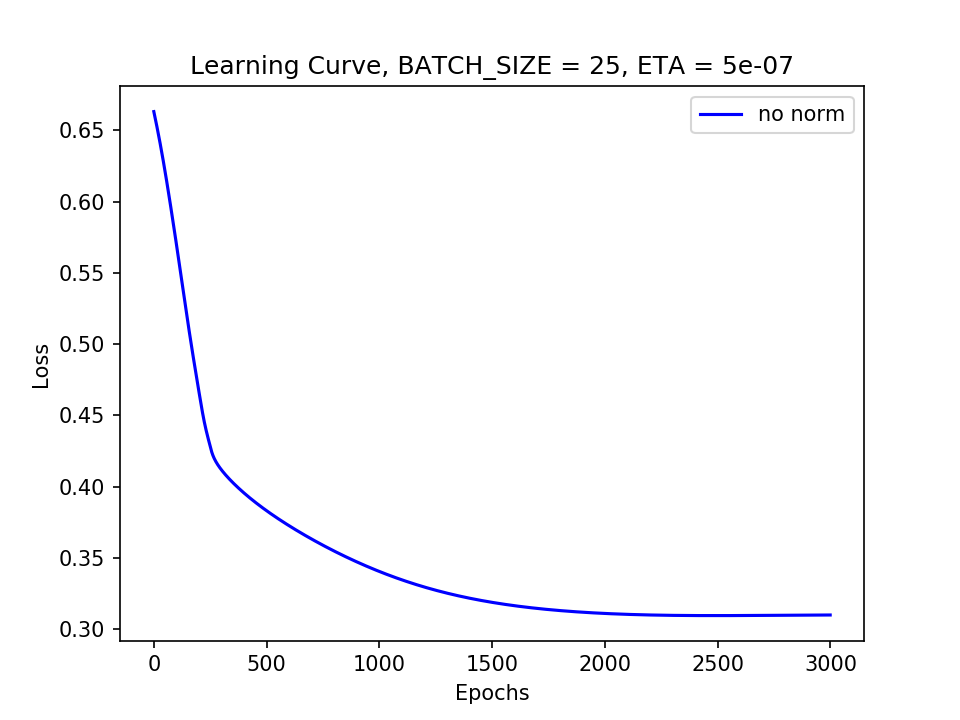
\includegraphics[scale = 1.0]{figure/LC_3.png}
\\ The Y-axis represents Loss, telling the learning curve(loss is dropping and finally converged)

\subsection{Training Error Rate} % Add another subsection
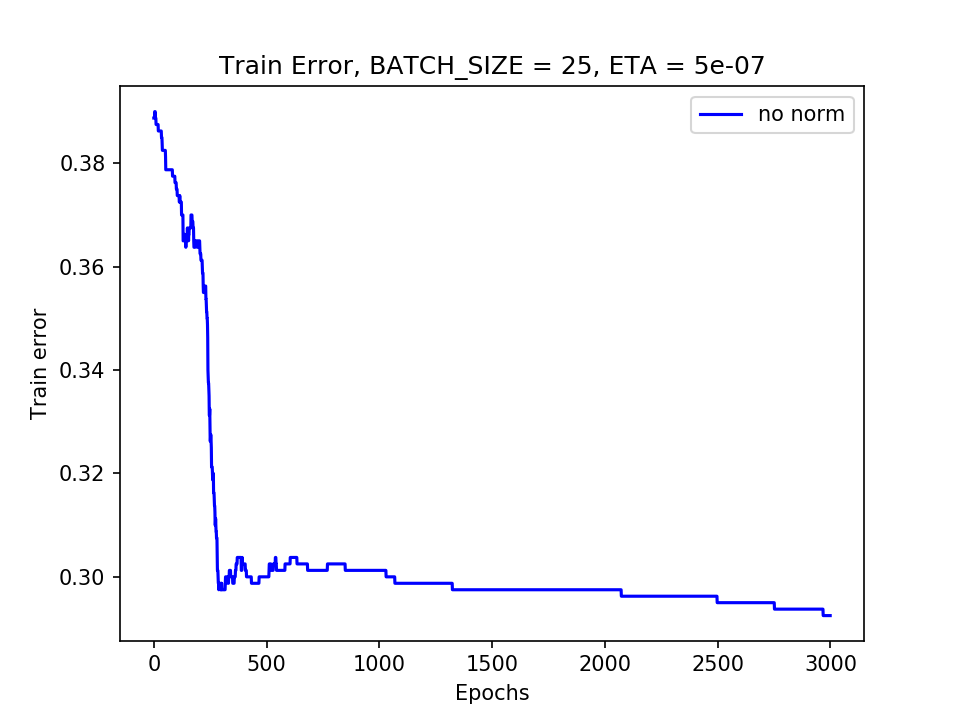
\includegraphics[scale = 0.8]{figure/TRE_3.png}
\\ The Y-axis represents training error rate, telling the error rate curve(error rate is dropping and finally converged)

\subsection{Testing Error Rate} % Add another subsection
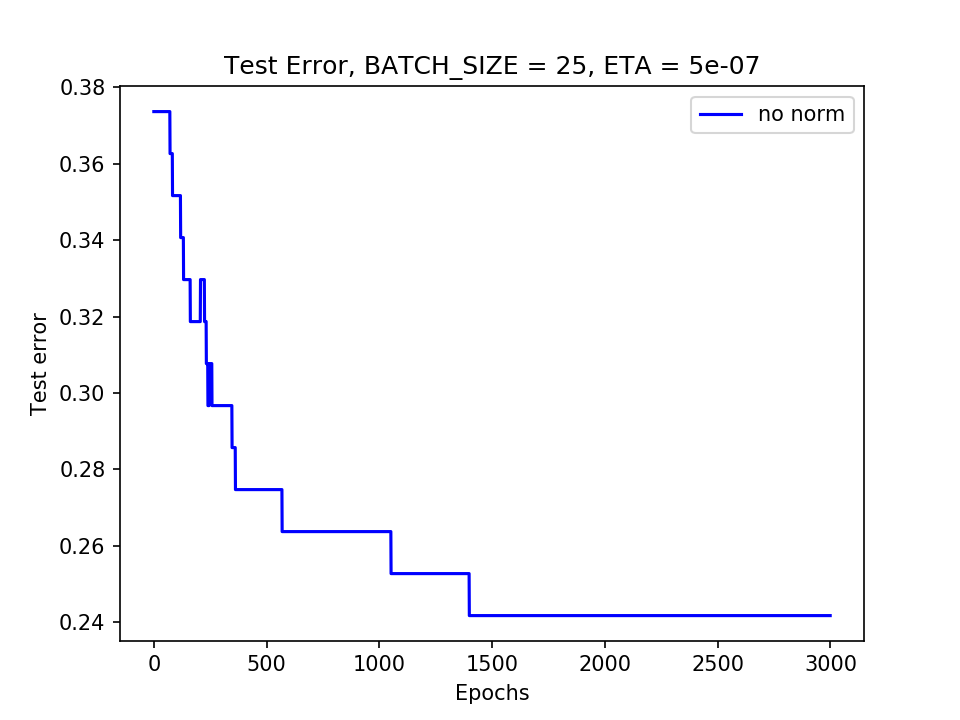
\includegraphics[scale = 0.8]{figure/TEE_3.png}
\\ The Y-axis represents testing error rate, telling the error rate curve(error rate is dropping and finally converged)

\subsection{Explanation of my neural network architecture} % Add another subsection
\begin{itemize}
    \item Layer: Input 6unit (input including 6 features, which is 6 dimensions). 
    \\ Hidden 4unit, since in my opinion, what influences the result most lies in the learning rate, the neuron set 4 will be optimal for computation (too many neurons merely increases the matrix computation time) 
    \\ \href{https://stats.stackexchange.com/questions/181/how-to-choose-the-number-of-hidden-layers-and-nodes-in-a-feedforward-neural-netw}{Click for ref}
    \\ Output: 1unit for alive or death.
    \\ For the following two items, I select them based on the combination with shell script, and comparing the optimal results using the \textbf{same random seed} for benchmarking the learning curve vs batch size and learning rate. (Choose the normal learning rate first (such as 0.5) and slightly decrease by empirical method (automated training with shell script and comparing with pyplot figure).
    \\ According to \href{https://medium.com/@chih.sheng.huang821/機器學習-基礎數學-三-梯度最佳解相關算法-gradient-descent-optimization-algorithms-b61ed1478bd7}{this article} the \textbf{high learning rate will cause the non-convergent of learning curve.}
    \\ With the aforementioned site, I start up with learning rate 0.5 and empirically dropped down to about \textbf{5e-6}
    
    
    \begin{lstlisting}[language = bash]
    if [ $sel -eq 1 ];
    then
        for batch_size in 4 8 16 20 25 32 40
        do
            for learning_rate in  0.0000001 0.0000003 0.0000005 0.000001 0.000003 0.000005
            do
                echo $learning_rate
                python3 dnn_1.py $1\_$batch_size\_$learning_rate $batch_size $learning_rate
            done
        done
    else
        #python3 dnn_1.py $1_16_0.00001 16 0.00001
    fi
    
    mkdir -p $1 #_P3
    mv $1*\.png $1/ #_P3/
    \end{lstlisting}
     
    \item Batch size: 25 for optimal, (too large will consume too much memory resource, and too small will cause the unstable learning curve. Although more randomness, less chance to converge)
    \\ \href{https://www.zhihu.com/question/32673260}{Ref link}
    \item Learning rate: 0.0000005 (5e-7) will be optimal (The above figures shows some high learning rate causing non-convergent of learning curve) 
    \begin{figure}
        \centering
        \begin{minipage}{0.5\textwidth}
            \centering
            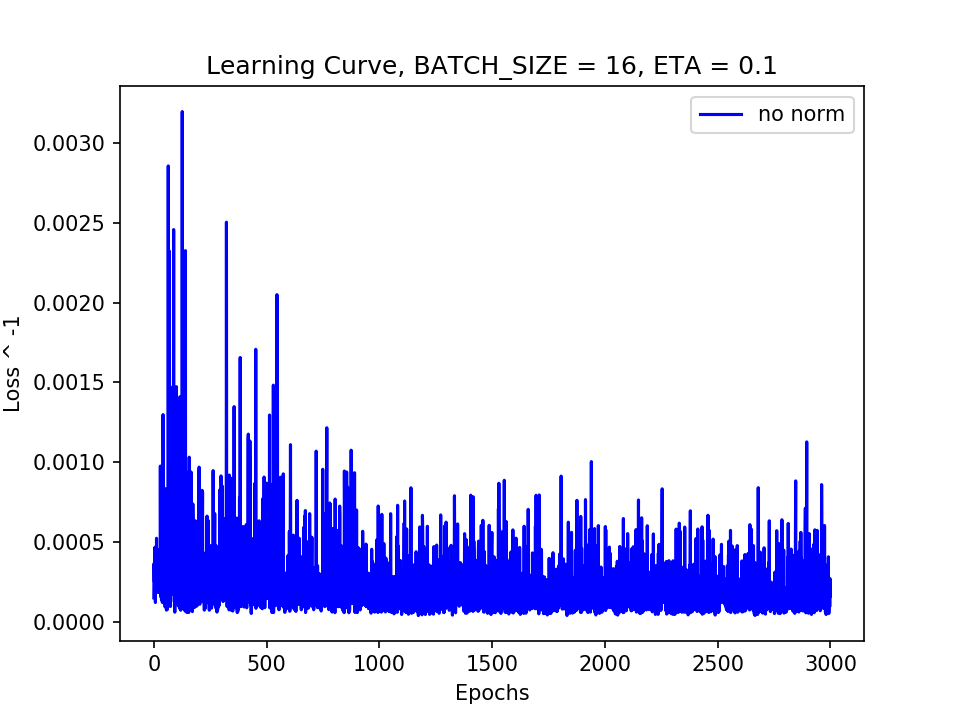
\includegraphics[width=0.9\textwidth]{figure/01_LC.png} % first figure itself
            \caption{Learning rate = 0.1}
        \end{minipage}\hfill
        \begin{minipage}{0.5\textwidth}
            \centering
            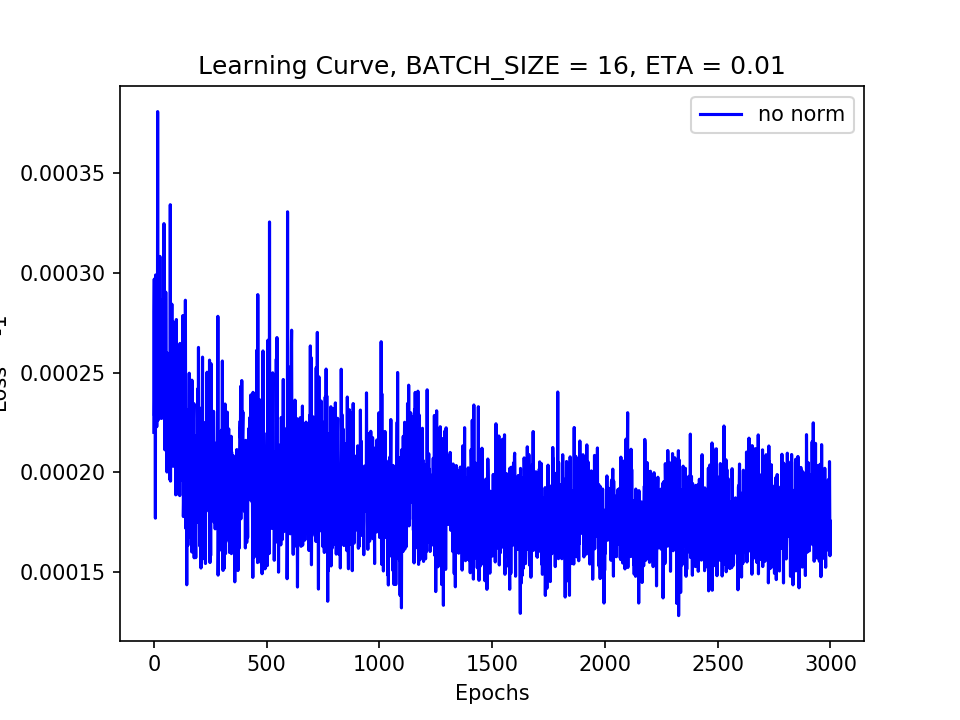
\includegraphics[width=0.9\textwidth]{figure/001_LC.png} % second figure itself
            \caption{Learning rate = 0.01}
        \end{minipage}
    \end{figure}
\end{itemize}
%----------------------------------------------------------------------------------------
% Literature review
%----------------------------------------------------------------------------------------

\section{TA-designed DNN}
The selection of learning rate and training batch size is the same as above
\\
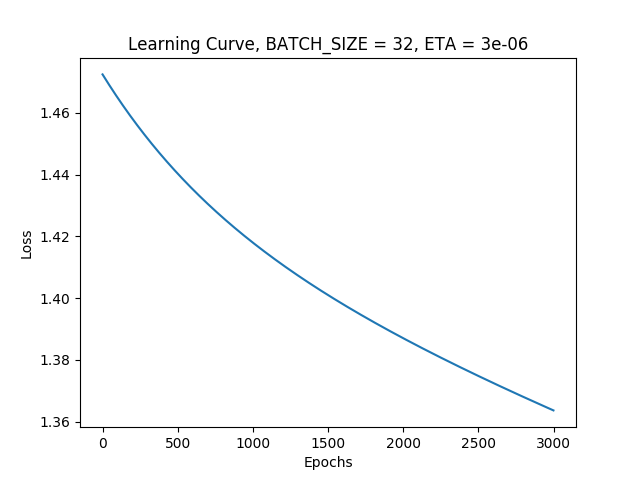
\includegraphics[scale = 0.6]{figure_2/LC.png} % first figure itself
\\
Learning curve
\\

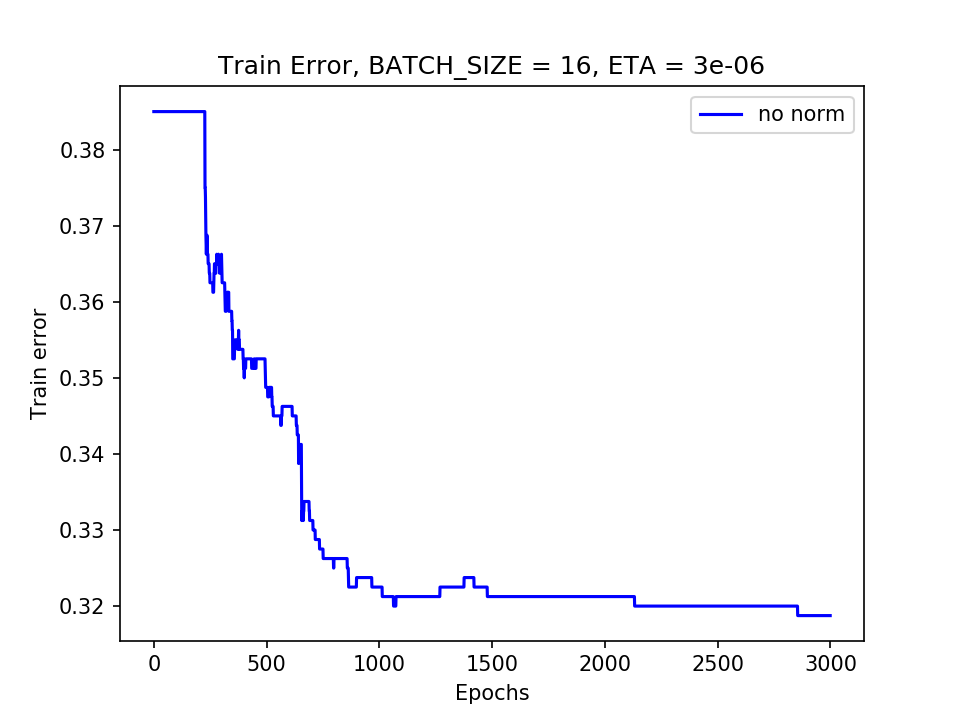
\includegraphics[scale = 0.6]{figure_2/TRE.png} % second figure itself
\\
Training error
\\

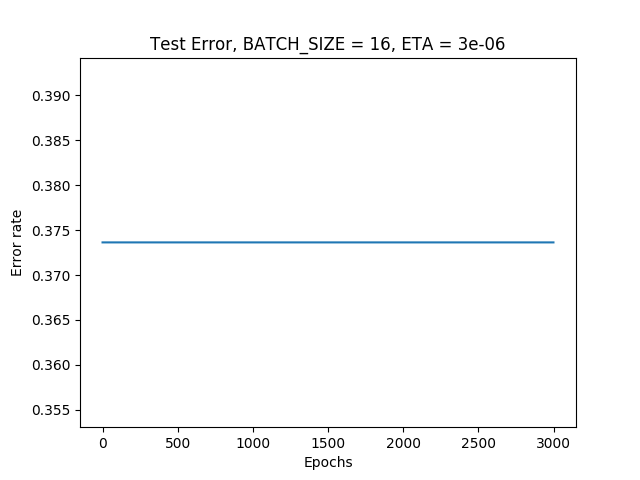
\includegraphics[scale = 0.6]{figure_2/TEE.png} % second figure itself
\\
Testing error
\\

\\ However, if we use the bigger batch size and higher learning rate, the result is totally different. especially in the train and test error rate. 
\\ 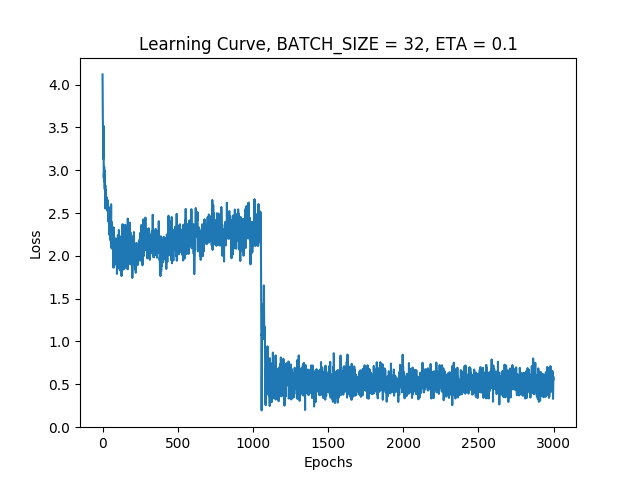
\includegraphics[scale = 0.6]{figure_2/LC_P2.png}
\\ 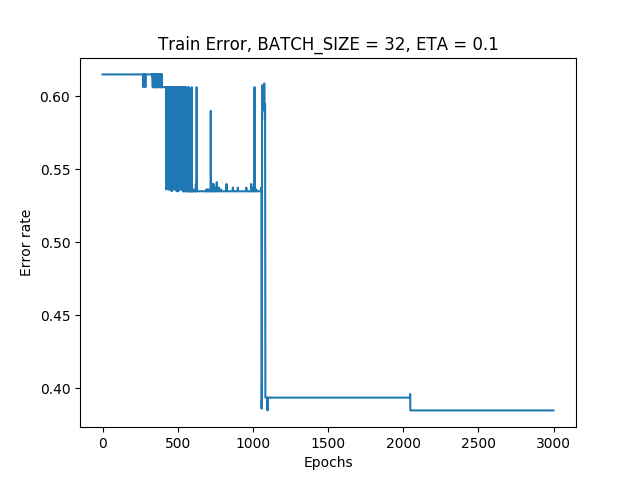
\includegraphics[scale = 0.6]{figure_2/TRE_P2.png}
\\ 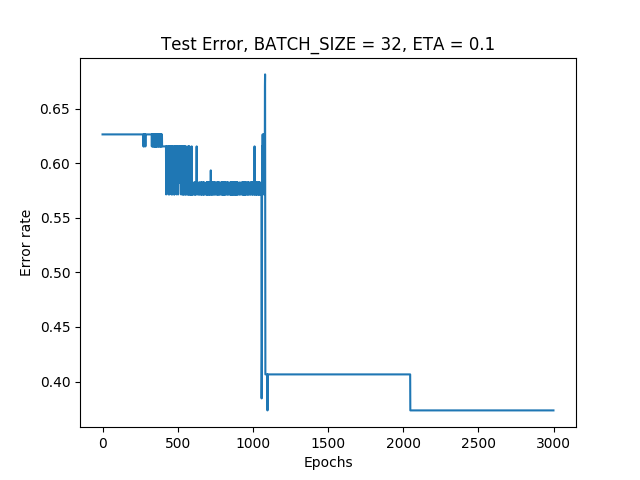
\includegraphics[scale = 0.6]{figure_2/TEE_P2.png}
\\ My speculation is that higher learning rate will learn faster undoubtedly but it also causes the unsuitability in the learning curve making it harder to converge. (Error rate drops quicker but oscillates) 

\section{The normalization of features}
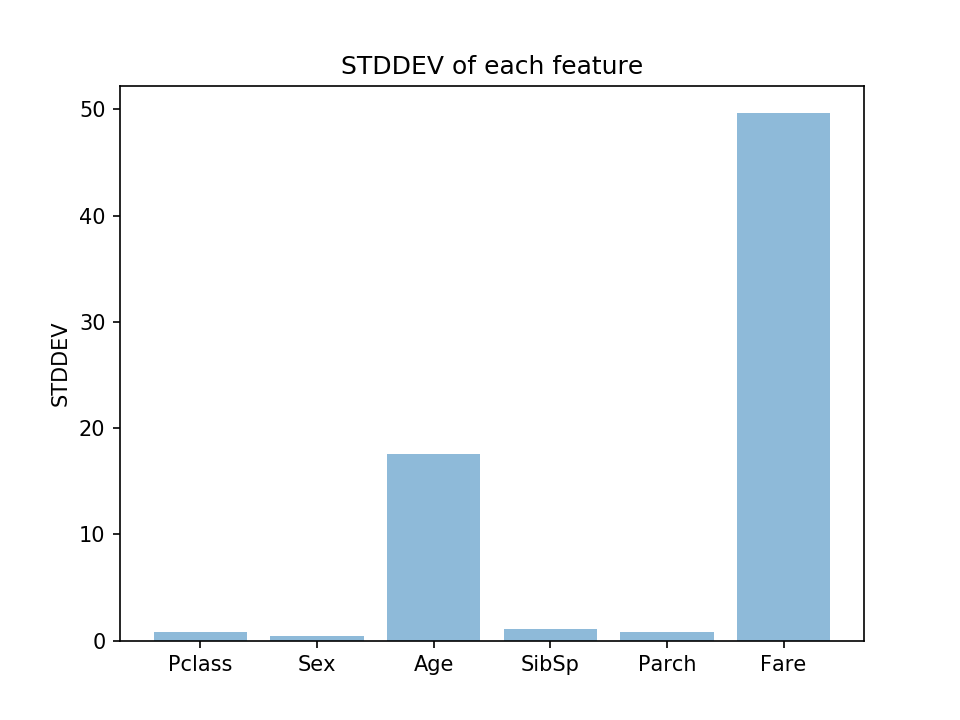
\includegraphics[scale = 0.7]{figure_2/STDDEV.png}
\\ Why normalize the data? 
\\ Normalization is a technique often applied as part of data preparation for machine learning. The goal of normalization is to change the values of numeric columns in the dataset to a common scale, without distorting differences in the ranges of values. For machine learning, every dataset does not require normalization. It is required only when features have different ranges.
\\ Aside from the 'fare' feature, the standard deviation of 'age' is big as well, hence for convenience and performance purpose, in the third test, I normalize all the classes.
\\ The following figure is the result of normalized fare and normalized all the features, which shows the better performance under normalization (use the same random seed, same batch size and same learning rate in whole program execution for fairness), the normalized results converged better and quicker . Note: Same cross entropy formula is used.
\\ 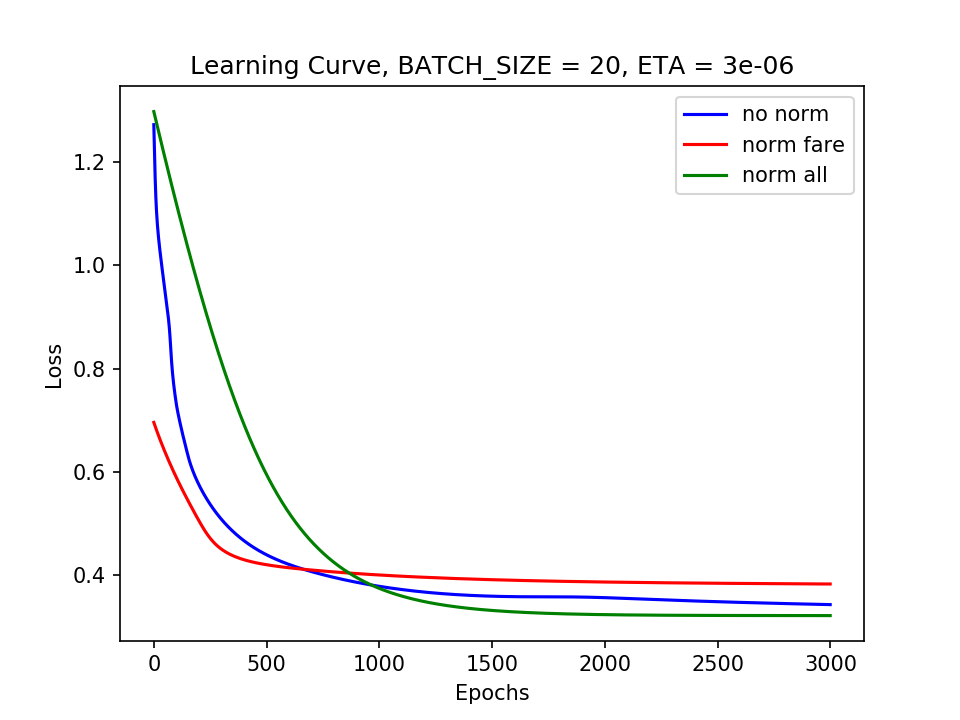
\includegraphics[scale = 0.5]{figure_2/NORM_LC.png}

\section{Feature that affects the prediction performance most}
By calculating the correlation coefficient for the feature vs output (alive or death), the following figure shows the \textbf{fare feature} affects the most (the higher the fare is, the more chance a passenger will survive).
\\ 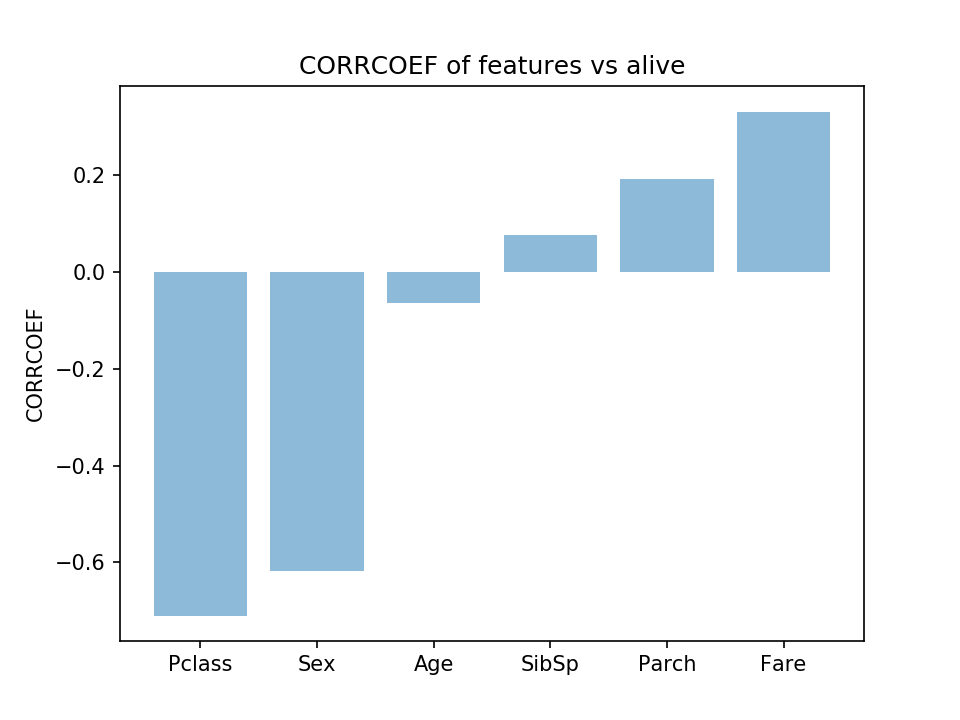
\includegraphics[scale = 1.0]{figure_2/CORRCOEF.png}

\section{Do we need one hot encoding?}
I downloaded the \textbf{full dataset from kaggle}, and use the dict to collect how many categories lies under the ticket class.
\\  It turns out to be that there are 594 difference b/w the training set and testing set by using the following code.
\begin{lstlisting}[language = python]
def parse(data):
    data = np.array(data)
    col = int(sys.argv[1])
    to_check = data[:,col]
    m = dict()
    for i in to_check:
        if i in m:
            m[i] += 1
        else:
            m[i] = 1
    for k, v in m.items():
        print(k, ' ', v)
    return m
def cmp_map(m1, m2):
    diff_dict = m1.keys() - m2.keys()
    print('Total differences ', len(diff_dict))

if __name__ == '__main__':
    label, train_data, test_data, all_data = file_IO()
    m1 = parse(train_data)
    m2 = parse(test_data)
    cmp_map(m1, m2)
\end{lstlisting}
\\ 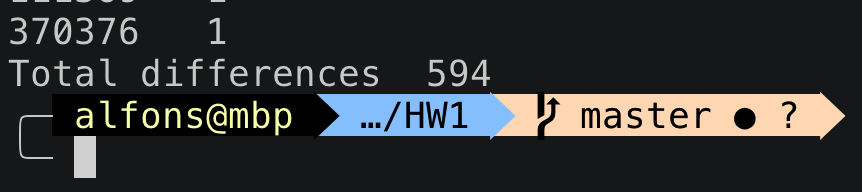
\includegraphics[scale = 0.5]{figure_2/diff.png}
\\ For the purpose of one-hot encoding, that is to \textbf{quantifies} the class since only some algorithms can work with categorical data directly. For example, a decision tree can be learned directly from categorical data with no data transform required (this depends on the specific implementation).
\\ Many machine learning algorithms cannot operate on label data directly. They require all input variables and output variables to be numeric.
\\ Nonetheless, in this dataset, the difference categories b/w the training set and testing set is 594 in the class 'ticket', rather big for merely a 91 testing set. Suppose on-hot encoding is used, each category is paired with an encoded data.
\\ For example, 2427 --> 001  5578 --> 010 7790 --> 100 308889 --> 101 in the training set. Due to so many different categories in the training set, this results in a big sparsity. 
\\ Suppose the testing set have input data somewhat like 'B2007T' or '8888' which none of them exists in the training set before, there will be no suitable data for NN to predict correctly
\\ \textbf{Unless further pre-processing is applied, one hot is not an idel choice here}

\section{Artificially design 2 samples for one alive and dead}
According to the covariance coefficient
\\ 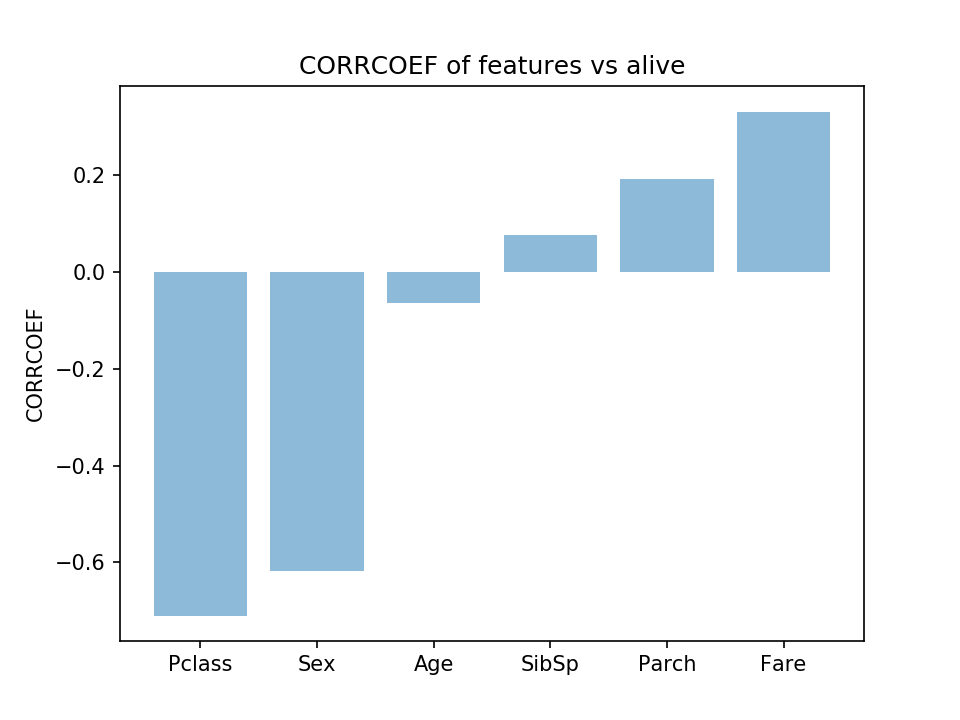
\includegraphics[scale = 0.7]{figure_2/CORRCOEF.png}
\\ What makes one survive the most is the 'fare' class and 'pclass', the former is positively related while the latter is negatively related. This means the more a passenger spends on the ticket and the less of pclass (kind like the first class, business and economy class in the plane), the more opportunity he/she will survive.
\\ Let the chance of survive > 0.5 as alive, otherwise dead to be the split line, here we have the artificially designed two samples for the problem.
\\ 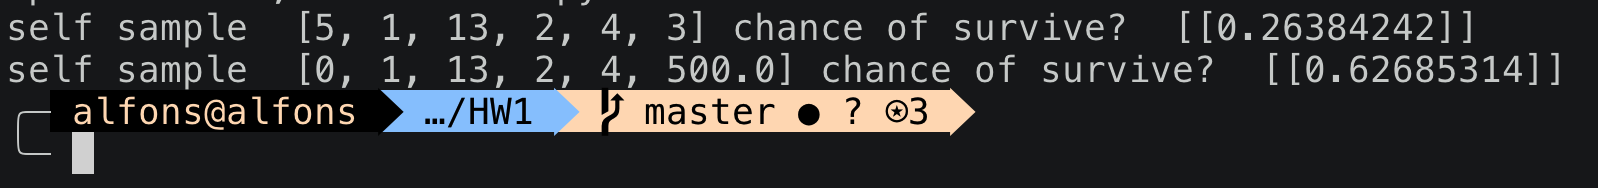
\includegraphics[scale = 0.5]{figure_2/survive.png}
\end{document}